\documentclass[12pt]{article}
\usepackage{graphicx}

\title{CarND Traffic Sign Classifier Project Writeup}
\author{Tiffany Huang}
\date{\today}

\begin{document}
\maketitle


\section{Traffic Sign Recognition Project}
This project consists on the following steps/tasks:
\begin{itemize}
\item{Load the data set}
\item {Explore, summarize, and visualize the data set.}
\item {Design, train, and test a model architecture}
\item {Use the model to make predictions on new images.}
\item {Analyze the softmax probabilities of the new images.}
\item {Summarize the results in a written report.}
\end{itemize}
My project code can be found here:

\section{Data Set Summary \& Exploration}
I used the \texttt{pandas} library to provide a summary of the data set. I found that the
\begin{itemize}
\item {Number of training examples = 34799}
\item {Number of validation examples = 4410}
\item {Number of testing examples = 12630}
\item {The shape of a traffic sign image was (26, 25)}
\item {Number of unique classes = 43}
\end{itemize}

\section{Exploratory Visualization of the Dataset}
To visualize the data, I used \texttt{matplotlib} to show the distribution of classes in the training, validation, and testing set. The histogram shows how many examples of each class exist in each dataset.
\begin{figure}[!h]
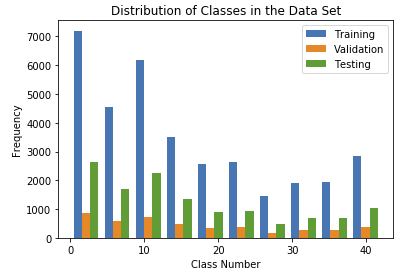
\includegraphics[scale=0.7]{writeup_images/distribution_classes.png}
\end{figure}

\section{Design and Test of a Model Architecture}
\subsection{Preprocessing}
The first step in my preprocessing was to grayscale the image because although colors can help determine the class of traffic sign, the shapes and gradients on the image are more reliable features that aren't subject to different lighting conditions. Here's an example of before and after grayscaling. The color is a bit off, but it's fixed after the normalization step at the end.
\begin{figure}[!h]
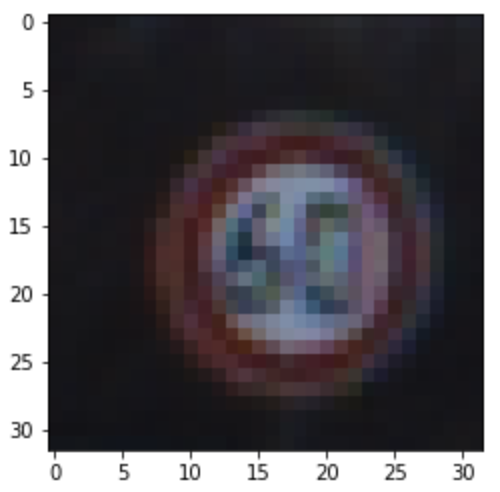
\includegraphics[scale = 0.5]{writeup_images/im1.png}
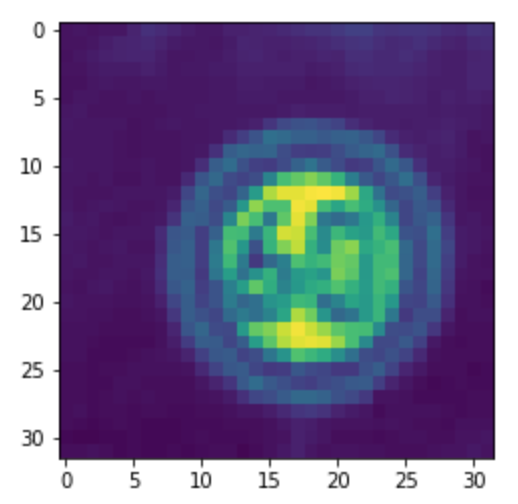
\includegraphics[scale = 0.5]{writeup_images/grayscale.png}
\end{figure}

Next, I cropped the image so that only the traffic sign is in the image. This step removes the background of the image, which in most cases does not provide any useful information to determine what kind of sign is in the image. For instance, grass does not help to indicate a stop sign vs. a general caution sign. By removing the excess information-lacking data allows the CNN to focus on the important features in the image. To do the cropping correctly, I had to resize the image to the original size because the bounding boxes for the signs were given with respect to the original image size. After the cropping, I then resized the image to 32 $\times$ 32 because my CNN takes this size image as input. An example is shown below:
\begin{figure}[!h]
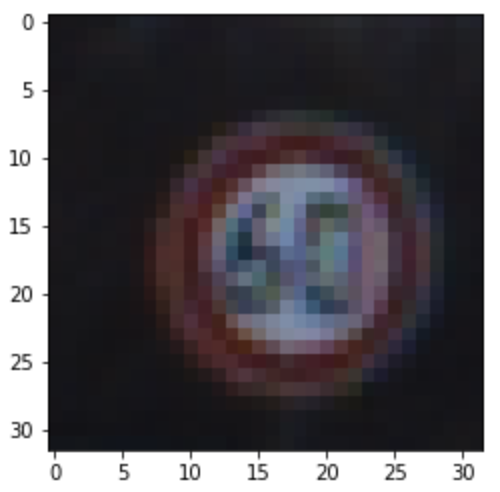
\includegraphics[scale = 0.5]{writeup_images/im1.png}
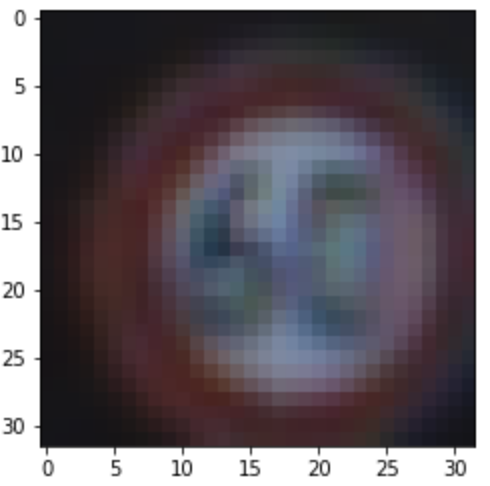
\includegraphics[scale = 0.5]{writeup_images/cropped.png}
\end{figure}

The next step was to normalize the image because different images were taken with different lighting, but different lighting should not affect the learned results. Thus, normalizing the image by subtracting the mean of the image and dividing by the standard deviation allows us to account for these environmental condition differences between images. I then layered this image into a 3 channel image with the same grayscale image in each channel to accommodate the input requirement of my CNN, which is a 32 $\times$ 32 $\times$ 3 image. An example of normalization is shown below:
\begin{figure}[!h]
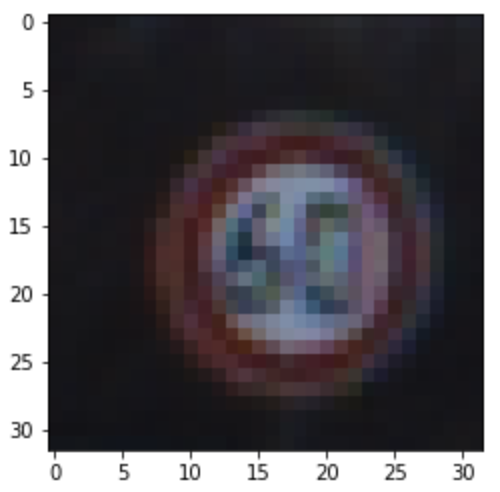
\includegraphics[scale = 0.5]{writeup_images/im1.png}
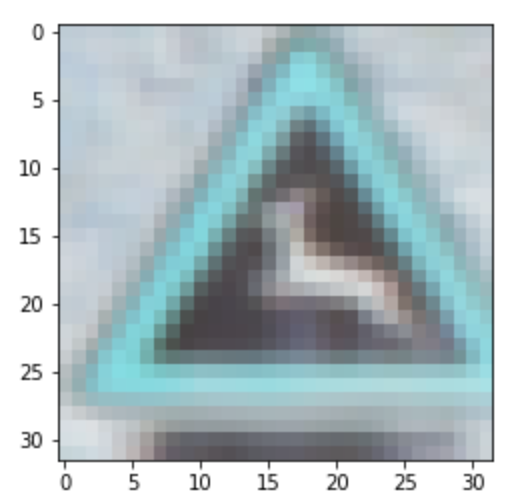
\includegraphics[scale = 0.5]{writeup_images/normalized.png}
\end{figure}

\subsection{Final Model Architecture}
My final model consists of the following layers:
\begin{center}
\begin{tabular}{|c|c|}
\hline
\textbf{Layer} & \textbf{Description} \\
\hline
Input & 32 x 32 x 3 RGB Image \\
\hline
Convolutional & 1 x 1 stride, VALID padding, outputs 30 x 30 x 4 \\
\hline
Activation & ReLU \\
\hline
Convolutional & 1 x 1 stride, VALID padding, outputs 29 x 29 x 5 \\
\hline
Activation & ReLU \\
\hline
Convolutional & 1 x 1 stride, VALID padding, outputs 28 x 28 x 6 \\
\hline
Activation & ReLU \\
\hline
Average pooling & 2 x 2 window, 2 x 2 stride, SAME padding, outputs 14 x 14 x 6 \\
\hline
Convolutional & 1 x 1 stride, VALID padding, outputs 10 x 10 x 16 \\
\hline
Activation & ReLU \\
\hline
Average pooling & 2 x 2 window, 2 x 2 stride, SAME padding, outputs 5 x 5 x 16 \\
\hline
Flatten & Outputs 400 x 1 \\
\hline
Fully connected & Outputs 300 x 1\\
\hline
Activation & ReLU \\
\hline
Dropout & Keep probability 0.8 \\
\hline
Fully connected & Outputs 200 x 1\\
\hline
Activation & ReLU \\
\hline
Dropout & Keep probability 0.8 \\
\hline
Fully connected & Outputs 120 x 1\\
\hline
Activation & ReLU \\
\hline
Dropout & Keep probability 0.8 \\
\hline
Fully connected & Outputs 84 x 1 \\
\hline
Activation & ReLU \\
\hline
Dropout & keep probability 0.8 \\
\hline
Fully connected & Outputs 43 x 1 \\
\hline
\end{tabular}
\end{center}

To train the model, I used a batch size of 128 with 10 epochs and an Adam optimizer with a learning rate of 0.001. The optimizer was trying to optimize the softmax cross entropy between the logits from the CNN and the one-hot encoded labels provided by the training set.

My final model results were a training accuracy of 0.975, a validation accuracy of 0.947, and a test set accuracy of 0.917. This is calculated in the \verb|evaluate(X_data, y_data, dropout_keep)| function which is called in the cell below it. The test accuracy is calculated in the "Predict the Sign Type for Each Image" section

I chose to use the LeNet architecture because it was originally used to classify numbers in an image. Since, traffic signs can also be classified based on similar features to numbers such as shapes (and some traffic signs even have numbers on them), I believed LeNet to be a good starting point for the traffic sign classification problem.

LeNet by itself could only achieve a validation accuracy of about 0.880, so I had to adjust the architecture a bit. The problem was overfitting because the training accuracy was about 0.1 higher than the validation accuracy. I added two convolutional layers on top of LeNet because traffic signs are generally more complicated than simple numeric digits. Additional convolutional layers allow the network to build up a more complex understanding of the image, combining simpler characteristics in earlier layers like basic lines and simple shapes to form a traffic sign. 

I changed the max pooling in the LeNet to average pooling because it seemed like max pooling could have been too much of a loss of information and average pooling could keep more of the data in the image while still preventing overfitting.

I also added one more fully connected layer and dropout layers after 3 of the 4 fully connected layers. Dropouts prevent overfitting because they randomly drop units from the network during training so that the final model isn't so heavily dependent on the training data. I tuned the keep unit probability for the dropout layers empirically by just testing a few to see which one achieved the best validation performance. I found that a keep probability of 0.8 worked the best.

\section{Testing a Model on New Images}

\section{Visualizing the Neural Network}

\bibliographystyle{abbrv}
\bibliography{main}

\end{document}
